\begingroup
\graphicspath{{../prob_4/Figures/}}
% Problem 4: Utterance Representations and SVM Classification

\subsection{Dataset and Preprocessing}
The audio dataset consists of 1,200 training utterances and 300 test utterances spanning 10 spoken-digit classes (0--9) recorded from multiple speakers. Each waveform was sampled at 16~kHz and segmented into non-overlapping 15~ms frames (240 samples per frame). For each frame a 40-bin mel-filterbank power spectrum was computed and converted to the log scale. The log scale is used because raw mel power can span roughly 13 orders of magnitude; converting to dB compresses this dynamic range to about 80~dB, yielding numerical values that are easier to model and compare.

After feature extraction each utterance is represented as a variable-length sequence of shape $(n_{\text{frames}},40)$. From the training set we found MAX\_FRAMES = 54 (used for subsequent padding/truncation); this value was computed using training data only to avoid test leakage.

\subsection{Part 1 — Baseline: Average Frame Method}
The baseline representation collapses an utterance into a single fixed-length vector by averaging all frame features across time, producing a 40-dimensional vector per utterance. This is the simplest fixed-length representation and discards all temporal dynamics. Classification was performed with an SVM using an RBF kernel (C=10, gamma="scale") trained on StandardScaler-normalized features.

The baseline SVM achieved 48.3\% test accuracy. Measured classifier timings were: Train: 117.8\,ms, Test: 18.8\,ms. The low accuracy is explained by the representation choice: averaging removes temporal order and thereby destroys information that distinguishes many digits. For example, digits whose discriminative cues are temporal (the order and timing of formant energy) can have very similar mean spectra even though they are perceptually different.

\subsection{Part 2 — AutoEncoder Utterance Representation}

\subsubsection{Padding and Flattening}
Utterances vary in length, so each sequence was padded with zero-frames up to MAX\_FRAMES=54 or truncated if longer. After padding each utterance becomes a fixed-size matrix of shape $54\times40$, which was flattened into a 2160-dimensional vector. Padding was determined using the training split only and applied identically to train and test to avoid leakage.

\subsubsection{AutoEncoder Architecture}
An autoencoder was trained to reconstruct the 2160-dimensional input. The encoder/decoder architecture is shown in Table~\ref{tab:p4_ae_arch}.

\begin{table}[H]
\centering
\caption{AutoEncoder architecture used for Problem 4.}
\label{tab:p4_ae_arch}
\begin{tabular}{ll}
	\toprule
Layer & Size \\
\midrule
Input & 2160 \\
Encoder FC + ReLU & 512 \\
Encoder FC + ReLU & 256 \\
	\textbf{Bottleneck FC + ReLU} & \textbf{128} \\
Decoder FC + ReLU & 256 \\
Decoder FC + ReLU & 512 \\
Output FC (linear) & 2160 \\
\bottomrule
\end{tabular}
\end{table}

The autoencoder was trained with mean-squared-error reconstruction loss using Adam (learning rate $1\times10^{-3}$), batch size 64 for 100 epochs. Input features were StandardScaler-normalized before training. The training loss fell rapidly during the first epochs (epoch 10: 0.209 $\rightarrow$ epoch 20: 0.137 $\rightarrow$ \ldots $\rightarrow$ epoch 100: 0.039), with steep early improvement and gradual convergence toward epoch 80--90.

\subsubsection{Feature Extraction and Classification}
After training, the 128-dimensional bottleneck activations were used as utterance feature vectors. An SVM with RBF kernel (C=10, gamma="scale") was trained on these latent vectors using StandardScaler normalization. The AE pipeline plus SVM achieved 93.3\% test accuracy. Measured classifier timings were: Train: 88.2\,ms, Test: 34.0\,ms. Note that AE training (several minutes on CPU) is a one-time preprocessing cost and is excluded from these classifier timings.

\subsection{Results}

\subsubsection{Summary Table}
The quantitative results are summarised in Table~\ref{tab:p4_summary}.

\begin{table}[H]
\centering
\caption{Problem 4 — Method comparison}
\label{tab:p4_summary}
\begin{tabular}{lccc}
	\toprule
Method & Accuracy & Train Time & Test Time \\
\midrule
Baseline (Average Frame) & 48.3\% & 117.8 ms & 18.8 ms \\
AE (Pad+Encode+SVM) & \textbf{93.3\%} & 88.2 ms & 34.0 ms \\
\bottomrule
\end{tabular}
\end{table}

Note: AE training time (several minutes on CPU) is a one-time preprocessing cost and is not included in the classifier timing numbers above.

\subsubsection{Figure 1 — Confusion Matrices}
\begin{figure}[H]
	\centering
	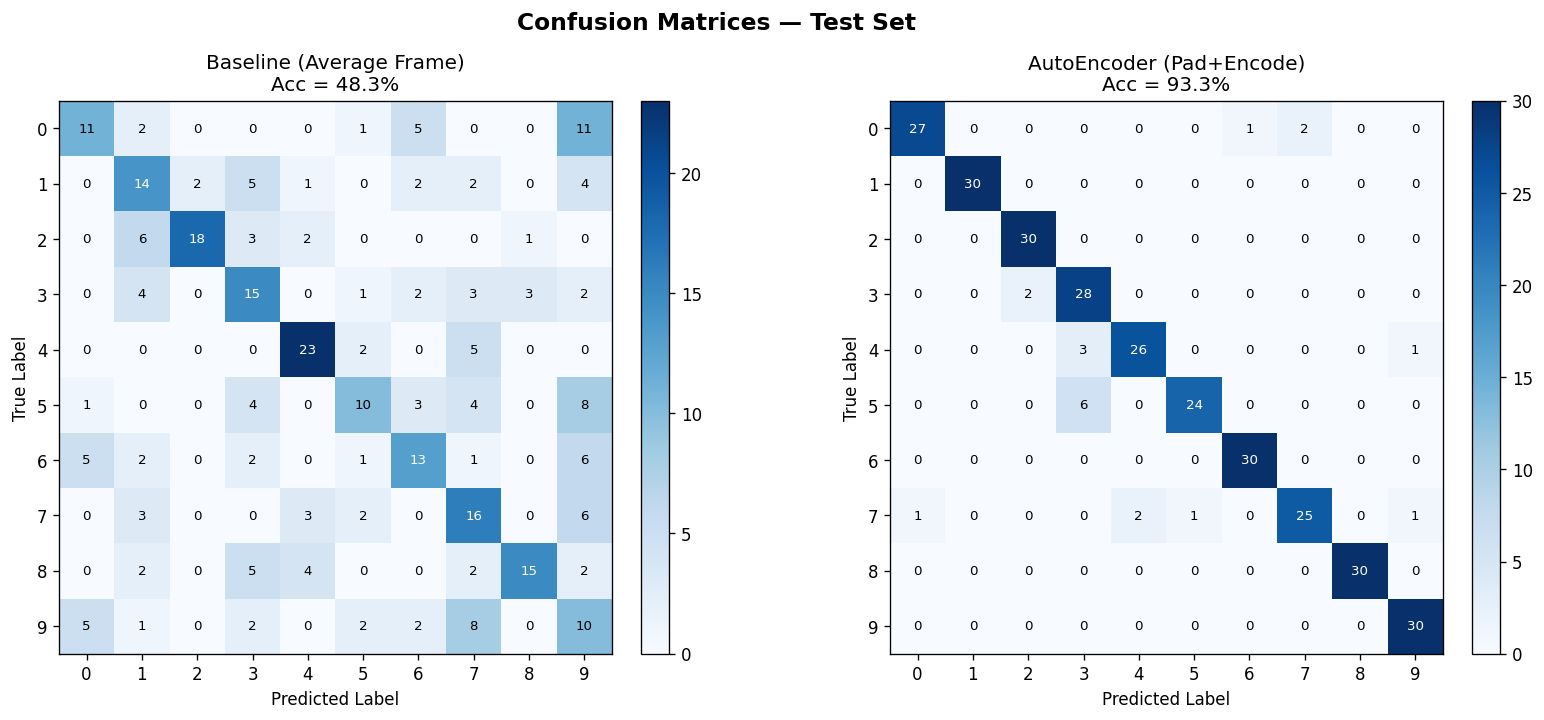
\includegraphics[width=0.9\textwidth]{confusion_matrices.png}
	\caption{Confusion matrices for the Baseline (left) and AE (right) systems.}
	\label{fig:p4_confusion}
\end{figure}

The baseline confusion matrix (left panel of Figure~\ref{fig:p4_confusion}) shows widely scattered predictions with only weak diagonal structure; many digits are confused with acoustically similar alternatives (for example, 5 and 9, 0 and 9). The AE confusion matrix (right panel) is nearly diagonal: most digits are classified correctly (25--30/30). Remaining errors are isolated: digit 5 has the most confusions (6 errors, mostly with digit 3), digit 7 has 5 errors, digit 4 has 4 errors, and digits 0 and 3 each have 3 errors (notably digit 0 is mislabelled as 6 and 7). These correspond to acoustically hard confusions.

\subsubsection{Figure 2 — Per-Digit Accuracy}
\begin{figure}[H]
	\centering
	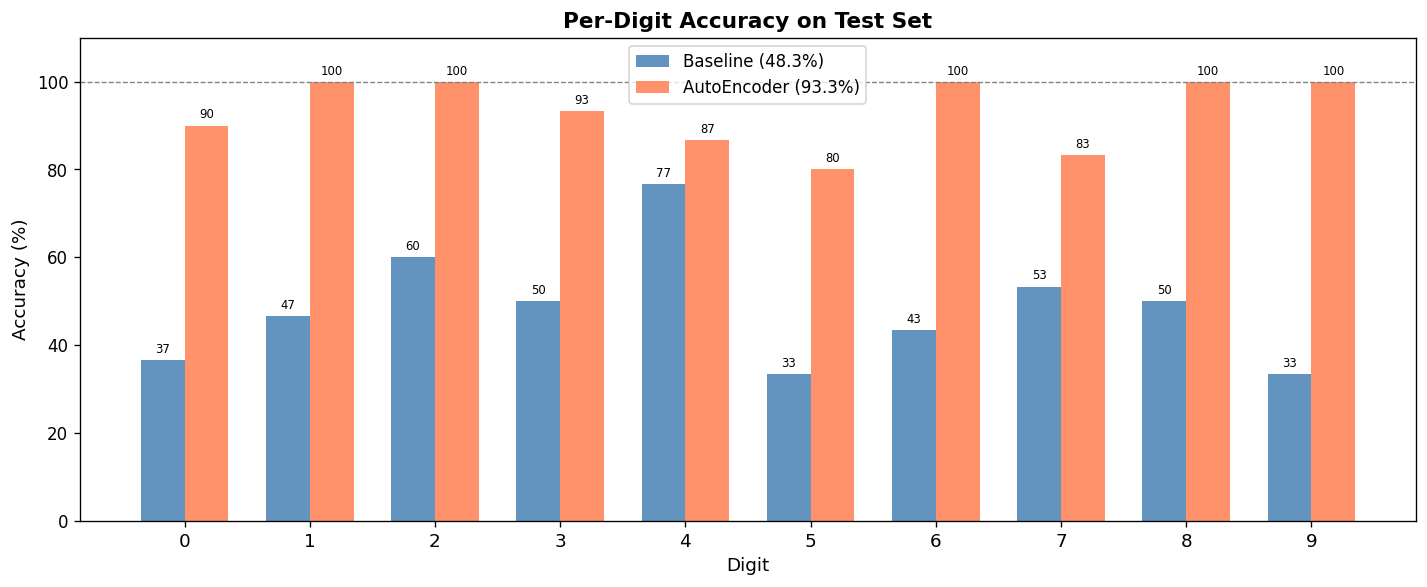
\includegraphics[width=0.8\textwidth]{per_digit_accuracy.png}
	\caption{Per-digit accuracy for Baseline and AE systems.}
	\label{fig:p4_perdigit}
\end{figure}

Figure~\ref{fig:p4_perdigit} shows per-digit accuracy. Under the baseline all digits fall between approximately 33\% and 77\% accuracy, with digits 5 and 9 worst (33\%) and digit 4 best (77\%). After AE encoding, digits 1, 2, 6, 8, and 9 reach 100\% accuracy; digits 0, 3, 4, and 7 lie in the 83--93\% range; digit 5 is the weakest at 80\%. The AE therefore raises the floor substantially — the weakest class jumps from 33\% to 80\%.

\subsection{Discussion}
Averaging frames fails because it discards temporal structure: the mean spectrum does not encode the order or timing of spectral events that distinguish many digit utterances. Consequently the baseline accuracy is low (48.3\%).

The autoencoder succeeds because by flattening a padded time sequence the encoder observes the full temporal trajectory and learns to compress discriminative temporal patterns into the 128-dimensional bottleneck. The resulting latent vectors are dense, discriminative, and compact, enabling an SVM to reach 93.3\% accuracy.

Timing-wise the SVM classifiers have similar train and test times (baseline ~118/19\,ms, AE ~88/34\,ms). The AE's training cost is a one-time expense that is amortised across inference calls; at test time the cost is an encoder forward pass plus an SVM prediction, which is negligible in most deployment scenarios.

Remaining errors concentrate on acoustically ambiguous digits (notably digit 5), consistent with confusions observed in Problem~3. Compared to the Problem~3 CNN baseline (95.3\%), the AE+SVM pipeline (93.3\%) attains comparable performance while being computationally lighter and simpler to run: no image rendering or 2D convolutions are required.

% End of Problem 4
\endgroup